\begin{multicols}{2}
\section{Digital vs. Analog}
Digital ist st"orsicher, hat keine St"orfortpflanzung und erlaubt einfachen Entwurf und Test mit Hilfe von CAD.

Analog ist st"oranf"allig, komplex, erfordert Spezialisten, Entwurf weitgehend von Hand, etc.

Digital ist aber langsamer, da alles in der Welt analog ist. F"ur Digital brauchts also noch eine Umwandlung.
\subsection{AD-Wandlung}
$$ \text{Abstastfrequenz} \geq 2\cdot f_{max}$$\\
$$ \Delta \text{Quantisierungsstufe} = 2 \cdot \text{Quantisierungsfehler}$$\\
$$\text{Amplitudenauflösung: Dynamik; SNR} \approx 6dB/bit$$
\end{multicols}

\begin{multicols}{2}
\section{Digital}
\subsection{FETs (selbstsperrend)}
	\begin{tabular}{|l|c|p{2.2cm}|p{2cm}|}
		\hline
		 & & $U_{GS}$ (leitend) & $I_D$ bei $U_{DS}$\\
		\hline
		n-FET & \raisebox{-.8\totalheight}{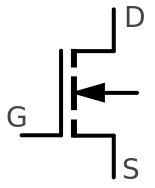
\includegraphics[width=0.05\textwidth]{pics/nFET}} & positiv & positiv \\
		\hline
		p-FET & \raisebox{-.8\totalheight} {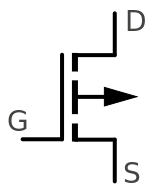
\includegraphics[width=0.05\textwidth]{pics/pFET}} & negativ & negativ \\
		\hline
	\end{tabular}
$$\hspace{-1.5cm}\text{Gatteräquivalent } n_{ge} = \frac{n_{trans}}{4}$$\\

\subsection{Zahlensysteme}
\subsubsection{Binär}
\paragraph{Bereichsüberschreitung Zweierkomplement}
\begin{itemize}
	\item [] Richtig $\Rightarrow Carry_n = Carry_{n-1}$\\
		  Falsch $\Rightarrow Carry_n \neq Carry_{n-1}$\\
\end{itemize}

\paragraph{Umwandeln von Komastellen}
\begin{itemize}
	\item [] $Komastelle_0 \cdot Basis = Ganzzahl_1,Komastelle_1$\\
		     $\dots$Weiterführen bis Genauigkeit erreicht ist\\		     
                     $Komastelle_{n-1} \cdot Basis = Ganzzahl_{n}, Komastelle_{n}$\\
			
	\item [] Wert hinter Koma in neuem Zahlensystem $= Ganzzahl_{1}\cdot Basis^{-1} + \dots+ Ganzzahl_n\cdot Basis^{-n}$\\
		Somit werden Stellen hinter Komma von oben nach unten aufgeschrieben

	\item [] \textbf{Beispiel} mit Zahl 2.7$_{10}$\\
		$\left.\begin{array}{ccc}
			2 / 2 & = 1 & R 0\\
			1 / 2 & = 0 & R 1
		\end{array}\right\uparrow$\\
		$\left.\begin{array}{cccl}
			0.7 \cdot 2 &= &\mathbf{1}.4\\
			0.4 \cdot 2 &= &\mathbf{0}.8\\
			0.8 \cdot 2 &= & \mathbf{1}.6\\
			0.6 \cdot 2 &= & \mathbf{1}.2\\
		\end{array}\right\downarrow$\\
		
		Zahl = 10,\textbf{1011}$\dots_2$ \\
	\end{itemize}
\end{multicols}
\vspace{-20pt}
